%%%%%%%%%%%%%%%%%%%%%%%%%%%%%%%%%%%%%%%%%
% Beamer Presentation
% LaTeX Template
% Version 1.0 (10/11/12)
%
% This template has been downloaded from:
% http://www.LaTeXTemplates.com
%
% License:
% CC BY-NC-SA 3.0 (http://creativecommons.org/licenses/by-nc-sa/3.0/)
%
%%%%%%%%%%%%%%%%%%%%%%%%%%%%%%%%%%%%%%%%%

%----------------------------------------------------------------------------------------
%	PACKAGES AND THEMES
%----------------------------------------------------------------------------------------

\documentclass{beamer}

\mode<presentation> {

% The Beamer class comes with a number of default slide themes
% which change the colors and layouts of slides. Below this is a list
% of all the themes, uncomment each in turn to see what they look like.

%\usetheme{default}
%\usetheme{AnnArbor}
%\usetheme{Antibes}
%\usetheme{Bergen}
%\usetheme{Berkeley}
%\usetheme{Berlin}
%\usetheme{Boadilla}
%\usetheme{CambridgeUS}
%\usetheme{Copenhagen}
%\usetheme{Darmstadt}
%\usetheme{Dresden}
%\usetheme{Frankfurt}
%\usetheme{Goettingen}
%\usetheme{Hannover}
%\usetheme{Ilmenau}
%\usetheme{JuanLesPins}
%\usetheme{Luebeck}
\usetheme{Madrid}
%\usetheme{Malmoe}
%\usetheme{Marburg}
%\usetheme{Montpellier}
%\usetheme{PaloAlto}
%\usetheme{Pittsburgh}
%\usetheme{Rochester}
%\usetheme{Singapore}
%\usetheme{Szeged}
%\usetheme{Warsaw}

% As well as themes, the Beamer class has a number of color themes
% for any slide theme. Uncomment each of these in turn to see how it
% changes the colors of your current slide theme.

%\usecolortheme{albatross}
\usecolortheme{beaver}
%\usecolortheme{beetle}
%\usecolortheme{crane}
%\usecolortheme{dolphin}
%\usecolortheme{dove}
%\usecolortheme{fly}
%\usecolortheme{lily}
%\usecolortheme{orchid}
%\usecolortheme{rose}
%\usecolortheme{seagull}
%\usecolortheme{seahorse}
%\usecolortheme{whale}
%\usecolortheme{wolverine}

%\setbeamertemplate{footline} % To remove the footer line in all slides uncomment this line
%\setbeamertemplate{footline}[page number] % To replace the footer line in all slides with a simple slide count uncomment this line

%\setbeamertemplate{navigation symbols}{} % To remove the navigation symbols from the bottom of all slides uncomment this line
}

\usepackage{graphicx} % Allows including images
\usepackage{booktabs} % Allows the use of \toprule, \midrule and \bottomrule in tables
\usepackage[francais]{babel}
\usepackage[utf8]{inputenc}
%----------------------------------------------------------------------------------------
%	TITLE PAGE
%----------------------------------------------------------------------------------------

\title[Sentiment analysis with RNN]{Analyse de sentiment par réseaux neuronaux réccurents} % The short title appears at the bottom of every slide, the full title is only on the title page

\author{Thomas Moreau \& Bertrand Rondepierre} % Your name
\institute[] % Your institution as it will appear on the bottom of every slide, may be shorthand to save space
{
Télécom paristech - MDI343 \\
}
\date{\today} % Date, can be changed to a custom date

\begin{document}

\begin{frame}
\titlepage % Print the title page as the first slide
\end{frame}

\begin{frame}
\frametitle{Overview} % Table of contents slide, comment this block out to remove it
\tableofcontents % Throughout your presentation, if you choose to use \section{} and \subsection{} commands, these will automatically be printed on this slide as an overview of your presentation
\end{frame}

%----------------------------------------------------------------------------------------
%	PRESENTATION SLIDES
%----------------------------------------------------------------------------------------

%------------------------------------------------
\section{Analyse de sentiment} % Sections can be created in order to organize your presentation into discrete blocks, all sections and subsections are automatically printed in the table of contents as an overview of the talk
%------------------------------------------------

%\subsection{Les objectifs}

%------------------------------------------------

\begin{frame}
\frametitle{Les Objectifs}
\begin{itemize}\setlength{\itemsep}{5mm}
\item Catégoriser l'opinion générale exprimée par une phrase
\item Plusieurs niveaux :
\begin{itemize}
\item Binaire : positif/négatif
\item Fine : Très négatif, négatif, neutre, positif, très positif
\end{itemize}
\item Représenter la phrase dans un espace propre qui permet de mettre en lumière l'opinion qu'elle contient
\item Génération de phrases ?
\end{itemize}
\end{frame}

%------------------------------------------------

\begin{frame}
\frametitle{Le Stanford Tree bank}
\begin{itemize}\setlength{\itemsep}{5mm}
\item 11 855 critiques de film issues de Rotten tomatoes
\item Structure de la phrase sous forme d'arbre et labels au niveau noeud\\
$\Rightarrow$ Possibilité d'analyse fine à chaque noeuds
\end{itemize}

\begin{figure}[htp]
\centering
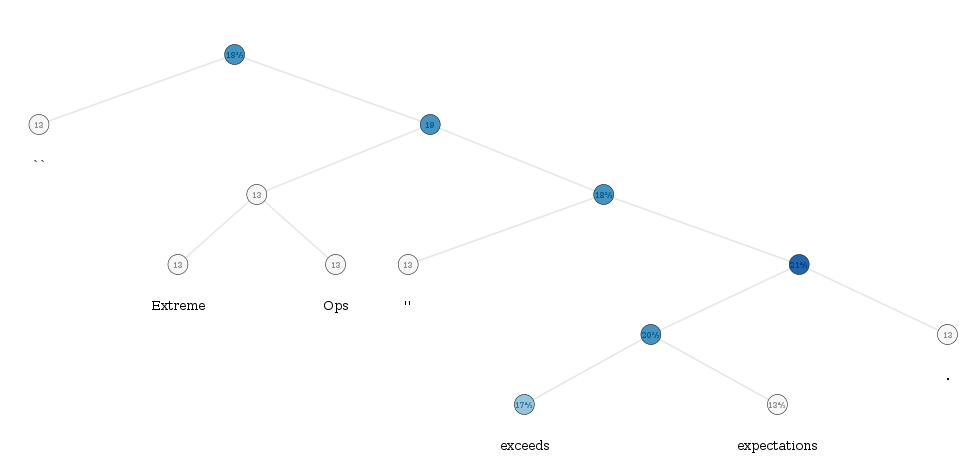
\includegraphics[scale=0.2]{fig/Tree10.png}
\caption{"Extreme Ops" exceeds expectations.}
\end{figure}

\end{frame}

%------------------------------------------------

\begin{frame}
\frametitle{Le modèle}
\begin{itemize}\setlength{\itemsep}{7mm}
\item \textbf{Classique}: Sac de mots - bag of word 
\item Ne tient pas compte de la structure de la phrase, seulement du nombre d'occurrences. 
\item Pourtant besoin de prendre en compte structure subtiles/fines : négation, expression etc...\\
\emph{This movie was actually neither that funny, nor super witty.}
\item Idée : utiliser la structure d'arbre pour prédire le sentiment à tous les niveaux de l'arbre, puis au niveau de la phrase complète.
\item On cherche aussi a optimiser la représentation des mots et phrases dans l'espace englobant.
\end{itemize}

\end{frame}

\begin{frame}
\frametitle{Réseau récurrent}
\begin{columns}
\begin{column}{0.45\textwidth}
Paramètres :
\begin{enumerate}
\item Dictionnaire des mots $L\in\mathbb{R}^{|V|\times d}$ 
\item $V\in\mathbb{R}^{d\times 2d\times 2d}$ le tenseur
\item $W\in\mathbb{R}^{d\times 2d}$ opérateur linéaire 
\item $W_s\in\mathbb{R}^{C\times d}$ softmax à chaque nœud où on fait une prédiction.
\end{enumerate}
\end{column}
\begin{column}{0.45\textwidth}
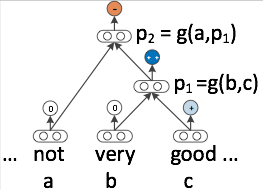
\includegraphics[width=\textwidth]{fig/RNN.png}
\end{column}
\end{columns}
\end{frame}

\begin{frame}
\frametitle{Réseau récurrent}
Forward pass (données $\rightarrow$ représentations + labels) :
\begin{enumerate}
\item L donne les représentation aux feuilles = mots
\item Pour deux enfants $i_1,i_2$ du nœud $i$ :
$$x^i=f\left(\begin{bmatrix} x^{i_1} \\ x^{i_2} \end{bmatrix}^T V^{[1:d]}\begin{bmatrix} x^{i_1} \\ x^{i_2} \end{bmatrix} + W\begin{bmatrix} x^{i_1} \\ x^{i_2} \end{bmatrix}\right)$$
Où $f$ est la fonction d'activation du réseau : $f=\tanh$ ici.
\item A chaque noeud où on dispose de la représentation $x^i$, softmax : $y^i=\sigma(W_s x^i)$ où :
$$\sigma_j(v)=\frac{\exp(v_j)}{\sum_{k=1}^C \exp(v_k)}$$
\end{enumerate}
\end{frame}
%------------------------------------------------
\section{L'apprentissage du modèle}

\begin{frame}
\frametitle{Fonction à optimiser}
Pour une distribution de proba cible $t^i$ au niveau du nœud $i$
\begin{itemize}\setlength{\itemsep}{4mm}
\item $ \displaystyle   E = \sum_{phrase}\sum_{nodes} D_{KL}(t^i||y^i)=\sum_{phrase}\sum_{nodes}\sum_{k}t^i_k \log y^i_k +C$.
\item Socher construit la distribution cible avec du one-hot encoding, ie binarise les 5 labels TN,N,Neutre,P,TP\\
$\rightarrow$ Pénalise de la même façon une erreur positif/très positif que très négatif/très positif.
\item Notre approche: 
\begin{itemize}
\item Approcher (KL) la probabilité $P[S=1]$ pour $S\in\{-1,1\}$ représentant le sentiment.
\item Construire la probabilité cible avec chaque sentiment représentant un niveau sur l'échelle $[0,1]$ (e.g neutre $=0.5$)
\end{itemize}
\end{itemize}
\end{frame}

%------------------------------------------------

\begin{frame}
\frametitle{Apprentissage}
\begin{itemize}
\item Rétropropagation des erreurs $\frac{\partial E^i}{\partial \theta} = (y^i-t^i)W_s\frac{\partial{x^i}}{\partial\theta} $:
\begin{align*}
	\frac{\partial{x^i}}{\partial\theta} &=F(x_j^i) \left( 2\begin{bmatrix} x^{i_g} \\ x^{i_d} \end{bmatrix}^T V^{[j]} +W_{j:}\right)\frac{\partial}{\partial\theta}\begin{bmatrix} x^{i_g} \\ x^{i_d} \end{bmatrix}
\\ &+ \begin{bmatrix} x^{i_g} \\ x^{i_d} \end{bmatrix}^T \frac{\partial V^{[j]}}{\partial\theta}\begin{bmatrix} x^{i_g} \\ x^{i_d} \end{bmatrix} + \frac{\partial W_{j:}}{\partial\theta}\begin{bmatrix} x^{i_g} \\ x^{i_d}\end{bmatrix}
\end{align*}
Pour le noeud $i$ avec $F$ telle que $F(f(x))=f'(x)$
\item Stratégie d'optimisation : AdaGrad \\
$\Rightarrow$ Principe : descente de gradient avec learning rate obtenu en diviser par la sommes des carrés des gradients déjà calculés. Favorise les features rare.
\item Autre solution: RPROP (resilient backpropagation) : \\
$\Rightarrow$ Augmentation/diminution multiplicative du learning rate en fonction de la dynamique du gradient.
\end{itemize}
\end{frame}

%------------------------------------------------
\section{Les résultats }

\begin{frame}
\frametitle{Paramètre}
\begin{itemize}
\item Learning rate, mini batch size, regularisation
\end{itemize}
\begin{figure}[htp]
\centering
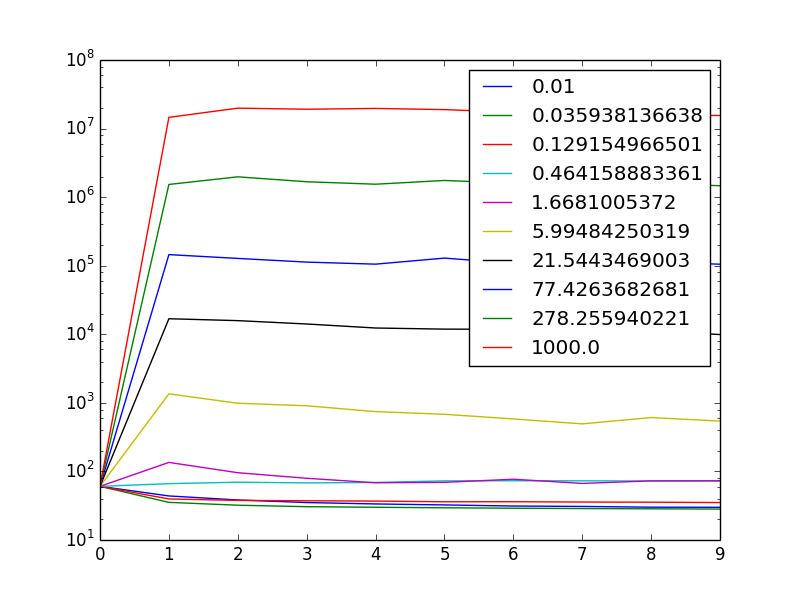
\includegraphics[scale=0.2]{fig/lr_curves.png}
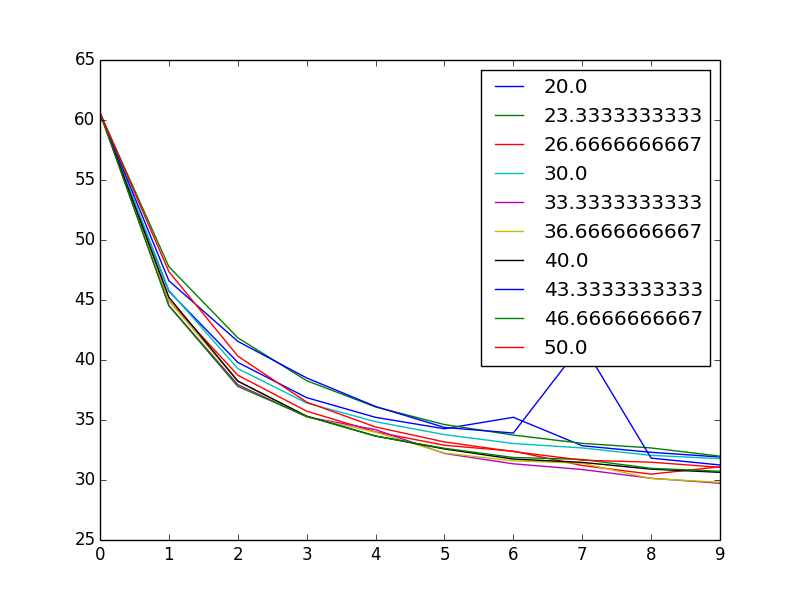
\includegraphics[scale=0.2]{fig/mb_curves.png}
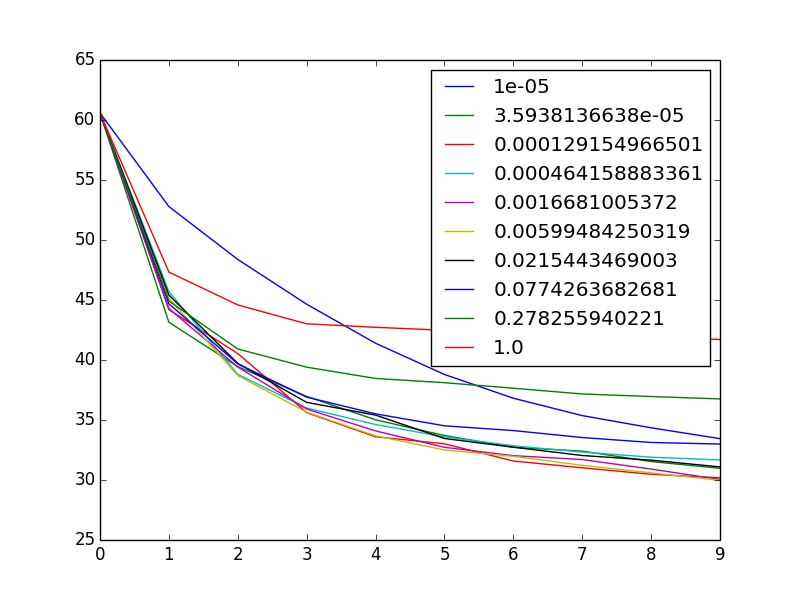
\includegraphics[scale=0.2]{fig/reg_curves.png}
\caption{Courbe d'apprentisssage en Cross validation pour le learning rate, la taille du mini batch et le facteur de régularisation}
\end{figure}

\end{frame}

%------------------------------------------------

\begin{frame}
\frametitle{Apprentissage}
\begin{figure}[htp]
\centering
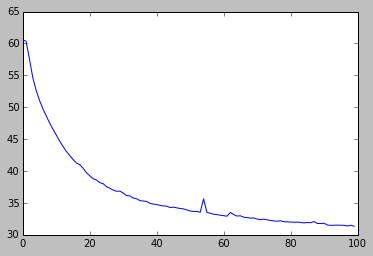
\includegraphics[scale=0.4]{fig/CourbeValAdaGrad.png}
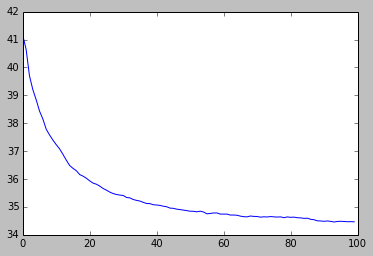
\includegraphics[scale=0.4]{fig/CourbeValRprop.png}
\caption{Courbe d'apprentisssage pour AdaGrad \emph{(gauche)} et Rprop \emph{(droite)}}
\end{figure}
Expérimentalement AdaGrad atteint un minimum local plus rapidement que Rprop qui se bloque beaucoup plus tôt.
\end{frame}

%------------------------------------------------

\begin{frame}
\frametitle{Resultat de Classification}
\begin{center}
\begin{tabular}{| c | c | c | c | c |}
\cline{2-5}
\multicolumn{1}{c}{} & \multicolumn{2}{| c |}{Fine} & \multicolumn{2}{| c |}{Binaire}\\\cline{2-5}
\multicolumn{1}{c |}{} & All node & Root & All nodes & Root \\\hline
Socher & 80.7  & 45.7 & 87.6 & 85.4\\\hline
Notre modèle & 79.7 & 42.2  & 86.6 & 90.6\\\hline
\end{tabular}
\end{center}

\begin{figure}[htp]
\centering
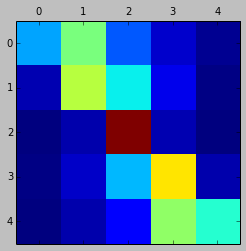
\includegraphics[scale=0.5]{fig/CMLastTrain.png}
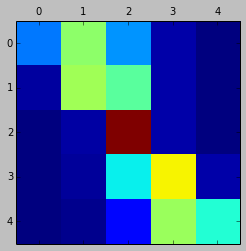
\includegraphics[scale=0.5]{fig/NewModelCFA.png}
\caption{Matrice de confusion Noeuds : Socher (gauche) nous (droite)}
\end{figure}

\end{frame}

\begin{frame}
\frametitle{Resultat de Classification}
\begin{center}
\begin{tabular}{| c | c | c | c | c |}
\cline{2-5}
\multicolumn{1}{c}{} & \multicolumn{2}{| c |}{Fine} & \multicolumn{2}{| c |}{Binaire}\\\cline{2-5}
\multicolumn{1}{c |}{} & All node & Root & All nodes & Root \\\hline
Socher & 80.7  & 45.7 & 87.6 & 85.4\\\hline
Notre modèle & 79.7 & 42.2  & 86.6 & 90.6\\\hline
\end{tabular}
\end{center}

\begin{figure}[htp]
\centering
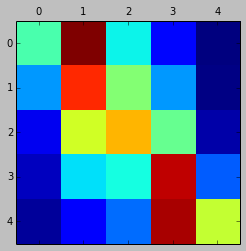
\includegraphics[scale=0.5]{fig/CMLastTrainRoot.png}
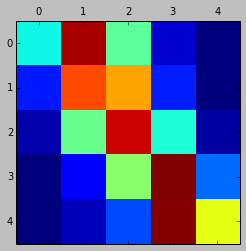
\includegraphics[scale=0.5]{fig/NewModelCFR.png}
\caption{Matrice de confusion racines : Socher (gauche) nous (droite)}
\end{figure}

\end{frame}

%------------------------------------------------

\begin{frame}
\frametitle{Résultat de Classification}
On représente pour notre modèle la précision en fonction de $\varepsilon$, ie le pourcentage de classification correcte avec des intervalles $|y^i-t^i|<\varepsilon$
\begin{figure}[htp]
\centering
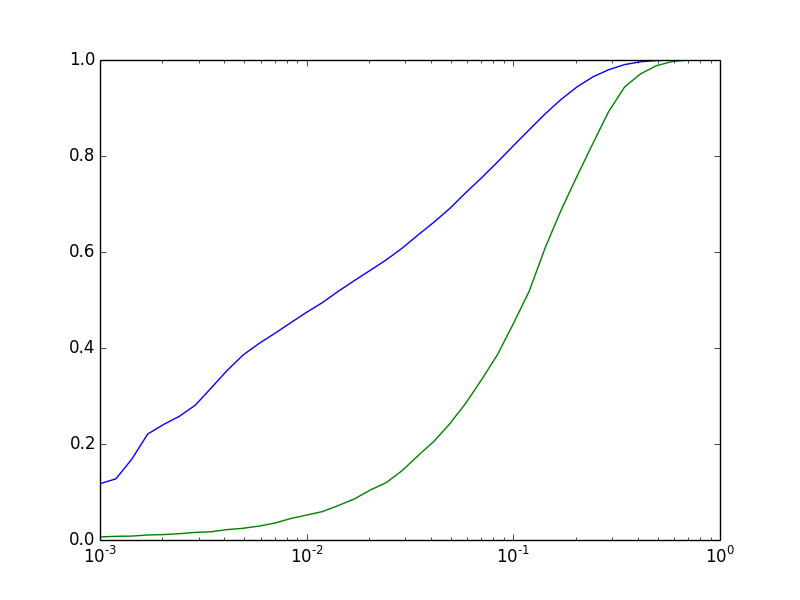
\includegraphics[scale=0.4]{fig/log_eps_curve.png}
\caption{Precision de notre regression (log scale)}
\end{figure}

\end{frame}


%------------------------------------------------

\begin{frame}
\frametitle{Représentations apprises - Mots}
\only<1> En représentant en 2D
\begin{figure}[htp]
\centering
\includegraphics<1->[width=0.45\textwidth]{fig/WordPlot.png}
\includegraphics<2>[width=0.45\textwidth]{fig/NewModelPCA.png}
\includegraphics<3>[width=0.45\textwidth]{fig/model2d.png}
\caption{\only<1>{PCA 2D du modèle de Socher}\only<2>{PCA de la représentation des mots en dimension 2. \hspace{\textwidth}.\hspace{0.1\textwidth}\emph{(gauche)} Socher 30D \emph{(droite)} Le nôtre 30D}\only<3>{Socher 30D \emph{(droite)} Le nôtre 2D}}
\end{figure}

\end{frame}
%------------------------------------------------

\begin{frame}
\frametitle{Représentations apprises - N-grams}
\begin{figure}[htp]
\centering
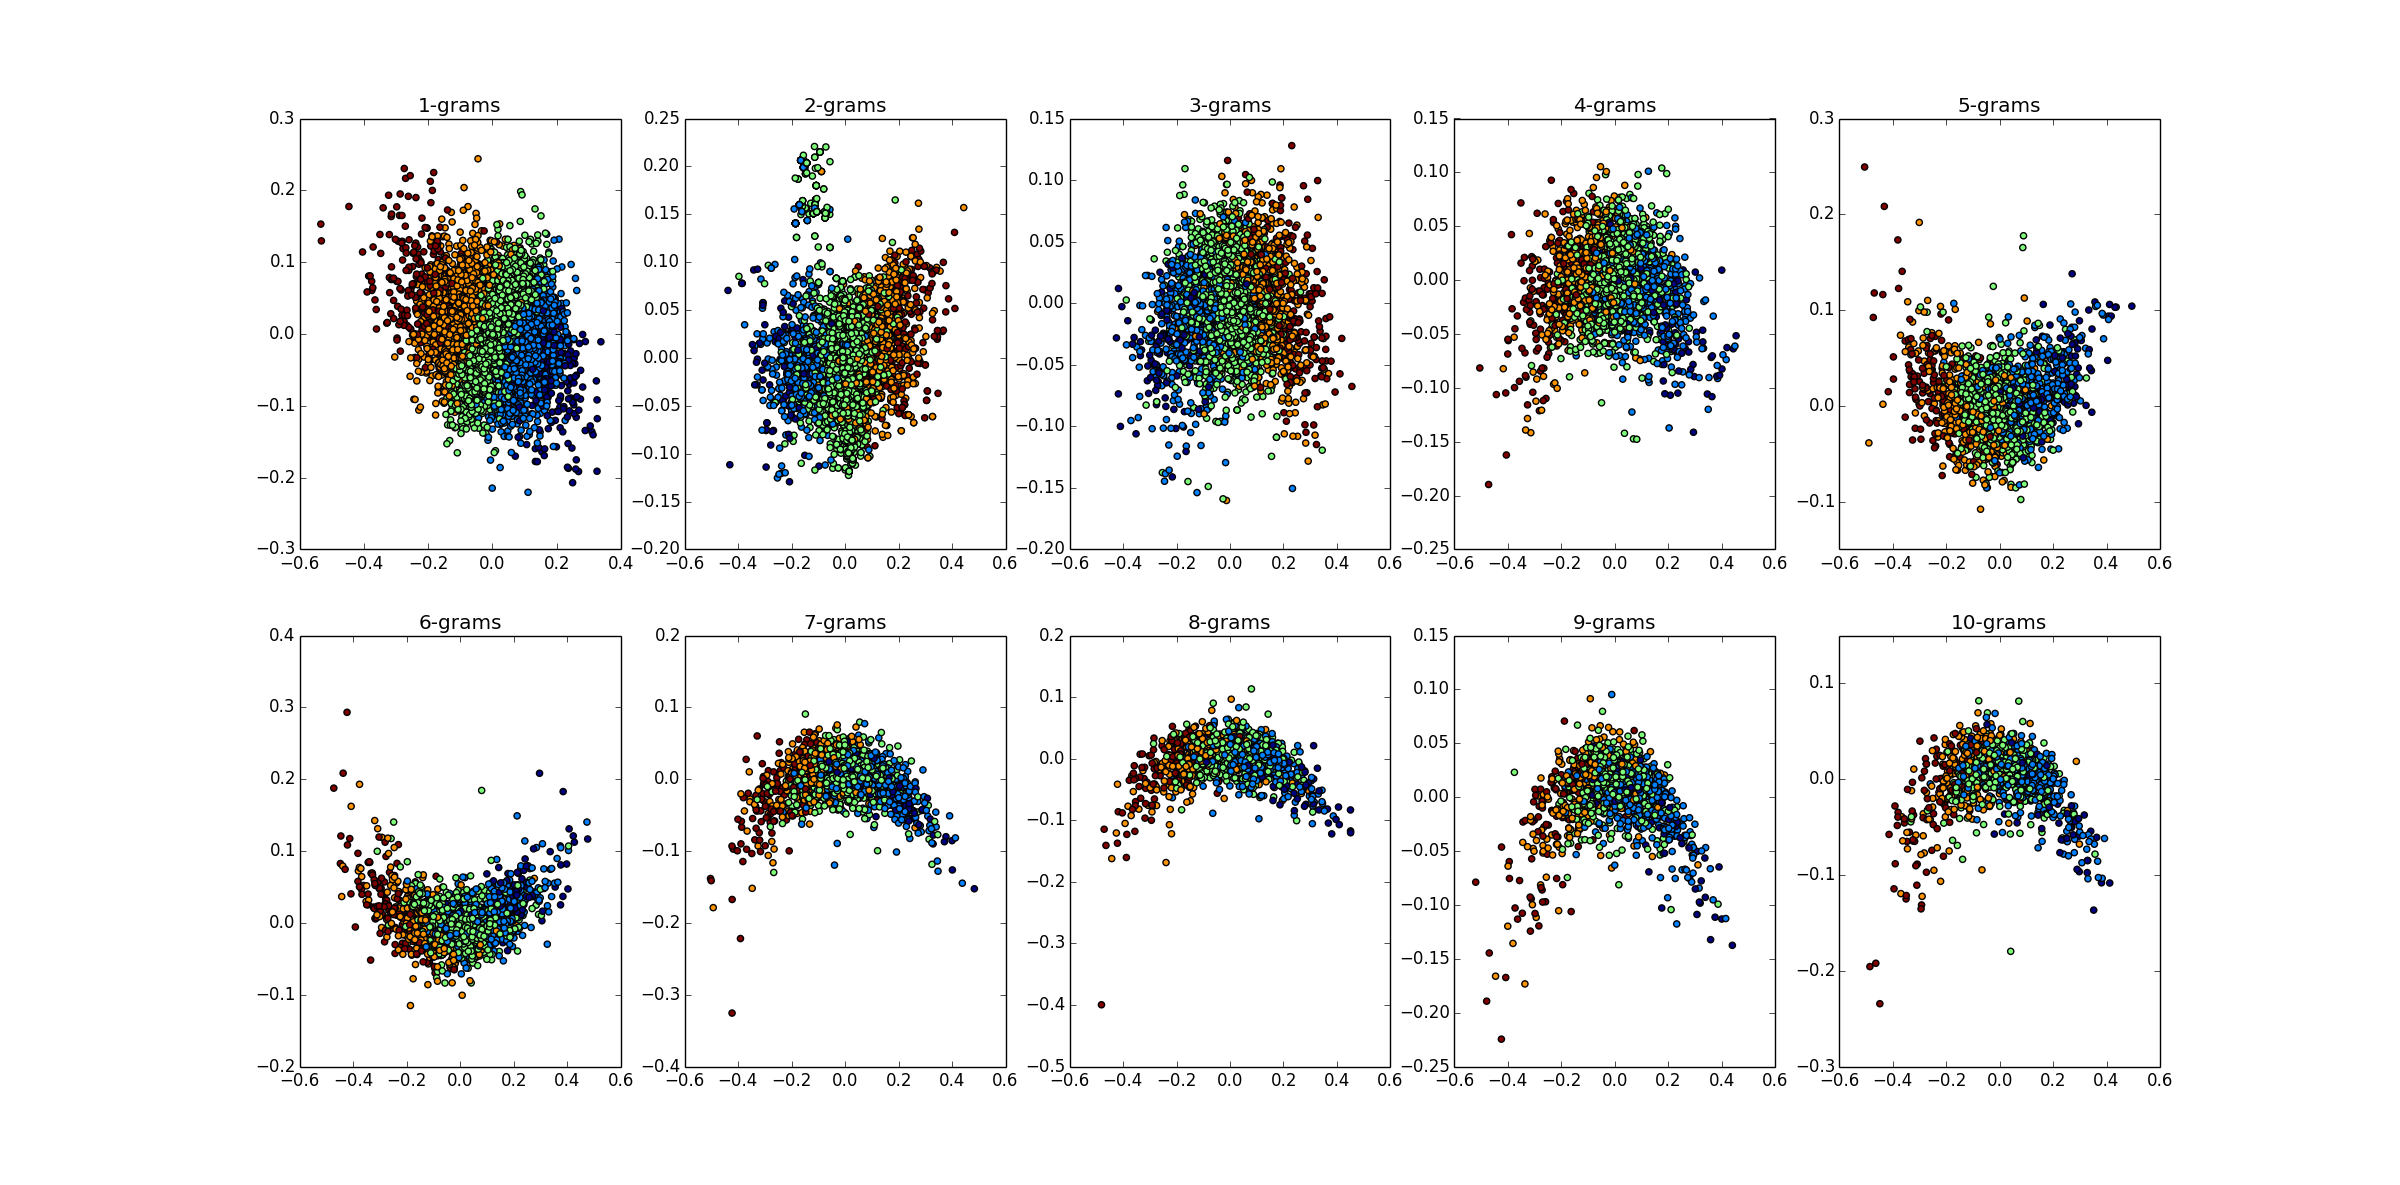
\includegraphics[scale=0.2]{fig/n_gram.png}
\caption[caption]{PCA de la représentation des mots en dimension 2 pour le modèle 30d}
\end{figure}
\end{frame}

%------------------------------------------------

\section{Auto encodeur}
\begin{frame}
\frametitle{Auto encodeur?}
\begin{itemize}
\item Idée : les figures précédentes suggère que l'on recombine mal les représentations.
\item Auto-encodeur optimise la reconstruction et peut espérer conserver la structure \\
$\Rightarrow$ Meilleure transmission de l'information ?
\item L'idée du modèle est
\begin{figure}[htp]
\centering
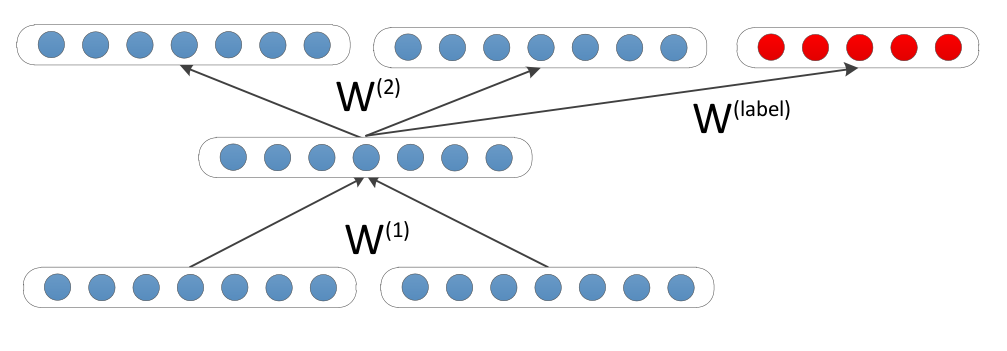
\includegraphics[scale=0.2]{fig/model_RAE.png}
\label{}
\end{figure}
\end{itemize}
\end{frame}

%------------------------------------------------

\begin{frame}
\frametitle{So far...}
\begin{itemize}\setlength{\itemsep}{5mm}
\item Back propagation découle de celle de notre modèle précédent
\item Ajout d'une dimension pour le sampling
\item Pour le moment, pas de structure, mais du sentiment.
\end{itemize}
\end{frame}


%------------------------------------------------

\begin{frame}
\Huge{\centerline{Question ?}}
\end{frame}

%----------------------------------------------------------------------------------------

\end{document} 